\documentclass{beamer}

\usepackage{../macros}

\title{Sort}

\begin{document}

\frame{
  \titlepage
}

\begin{frame}{Popular sorting algorithm}

  \begin{block}{}
    \begin{itemize}
      \item \only<2>\emphr{Insertion sort}
      \item Selection sort
      \item Bubble sort
      \item \only<2>\emphr{Merge sort}
      \item Quicksort
    \end{itemize}
  \end{block}
\end{frame}

\begin{frame}[fragile]{Insertion sort}
  \begin{block}{Using arrays}
    \centering
    \begin{tikzpicture}[scale = 0.5]
      \draw (0, 0) rectangle (5, 1);
      \foreach \x in {1, 2, ..., 5}
        \draw (\x, 0) -- (\x, 1);
        
      \draw (0.5, 0.5) node {1};
      \draw (1.5, 0.5) node {\only<-3>{\only<2>\emphr{5}}\only<4->{\only<4>\emph{3}}};
      \draw (2.5, 0.5) node {\only<-3>{\only<3>\emphr{3}}\only<4-6>{\only<4>\emph{5}}\only<7->{\only<7>\emph{4}}};
      \draw (3.5, 0.5) node {\only<-6>{\only<5>\emphr{6}}\only<7->{\only<7>\emph{5}}};
      \draw (4.5, 0.5) node {\only<-6>{\only<6>\emphr{4}}\only<7->{\only<7>\emph{6}}};
      
      \only<2>{\draw[rose, thick] (0, 0) rectangle (1, 1);}
      \only<3>{\draw[rose, thick] (0, 0) rectangle (2, 1);}
      \only<4-5>{\draw[rose, thick] (0, 0) rectangle (3, 1);}
      \only<6>{\draw[rose, thick] (0, 0) rectangle (4, 1);}
      \only<7>{\draw[rose, thick] (0, 0) rectangle (5, 1);}
    \end{tikzpicture}
  \end{block}
  
  \uncover<9->{
  \begin{block}{Using linked lists}
    \centering
    \begin{tikzpicture}[scale = 0.5]
%      \draw (2.5, 5) 
      \draw (0.5, 0) rectangle (1.5, 1) (0.5, 0) -- (1.5, 1) (0.5, 1) -- (1.5, 0);
      
      \uncover<-10>{\draw[->] (-1.5, 0.5) -- (0.25, 0.5);}
      
      \uncover<10->{
      \draw (0, -1.5) rectangle (2, -0.5) (1, -0.5) -- (1, -1.5);
      \draw (0.5, -1) node {3};
      \fill (1.5, -1) circle (2pt);
      }
      
      \only<11-14>{\draw[->, rounded corners] (-1.5, 0.5) -|  (-0.875, -1) -- (-0.25, -1);}
      \only<11-12>{\draw[->, rounded corners] (1.5, -1) -|  (2.5, 0.5) -- (1.75, 0.5);}
      
      \uncover<12->{
      \draw (3, -1.5) rectangle (5, -0.5) (4, -0.5) -- (4, -1.5);
      \draw (3.5, -1) node {5};
      \fill (4.5, -1) circle (2pt);
      }
      
      \uncover<13->{\draw[->, rounded corners] (4.5, -1) |- (1.75, 0.5);}
      \uncover<13-16>{\draw[->] (1.5, -1) -- (2.75, -1);}
      
      \uncover<14->{
      \draw (-0.5, -3) rectangle (1.5, -2) (0.5, -2) -- (0.5, -3);
      \draw (0, -2.5) node {1};
      \fill (1, -2.5) circle (2pt);
      }
      
      \only<15->{\draw[->, rounded corners] (-1.5, 0.5) -|  (-1.125, -2.5) -- (-0.75, -2.5);}
      \only<15->{\draw[->, rounded corners] (1, -2.5) |-  (-0.75, -1.75) |- (-0.25, -1);}
      
      \uncover<16->{
      \draw (2.5, -3) rectangle (4.5, -2) (3.5, -2) -- (3.5, -3);
      \draw (3, -2.5) node {4};
      \fill (4, -2.5) circle (2pt);
      }
      
      \only<17->{\draw[->, rounded corners=2] (1.5, -1)  -- (1.5, -1.75) --  (1.875, -1.75) -- (1.875, -2.5) -- (2.25, -2.5);}
      \only<17->{\draw[->, rounded corners] (4, -2.5) |-  (2.25, -1.75) |- (2.75, -1);}
      
      
    \end{tikzpicture}
  \end{block}}
\end{frame}

\begin{frame}{Merge sort}
  
  \begin{block}{Merging two sorted arrays}
    \centering
    \begin{tikzpicture}[scale = 0.45]
      \draw (0, 0) rectangle (3, 1);
      \draw (0, -2) rectangle (3, -1);
      \foreach \x in {1, 2} {
        \draw (\x, 0) -- (\x, 1);
        \draw (\x, -2) -- (\x, -1);
      }
      
      \draw (0.5, 0.5) node {\only<3-4>\emphr{\only<5->\info{1}}};
      \draw (1.5, 0.5) node {\only<5-8>\emphr{\only<9->\info{3}}};
      \draw (2.5, 0.5) node {\only<9-10>\emphr{\only<11->\info{5}}};
      
      \draw (0.5, -1.5) node {\only<3-6>\emphr{\only<7->\info{2}}};
      \draw (1.5, -1.5) node {\only<7-12>\emphr{\only<13->\info{7}}};
      \draw (2.5, -1.5) node {\only<13-14>\emphr{\only<15->\info{9}}};
      
      \uncover<2->{
        \draw (-1.5, -4.5) rectangle (4.5, -3.5);
        \foreach \x in {-0.5, 0.5, ..., 3.5}
          \draw (\x, -4.5) -- (\x, -3.5);
      }
      \only<4->{\draw (-1, -4) node {\only<4>\emph1};}
      \only<6->{\draw (0, -4) node {\only<6>\emph2};}
      \only<8->{\draw (1, -4) node {\only<8>\emph3};}
      \only<10->{\draw (2, -4) node {\only<10>\emph5};}
      \only<12->{\draw (3, -4) node {\only<12>\emph7};}
      \only<14->{\draw (4, -4) node {\only<14>\emph9};}
    \end{tikzpicture}
  \end{block}
  
\end{frame}

\begin{frame}{Merge sort}

  \begin{block}{Dichotomic sort}
    \centering
    \begin{tikzpicture}[scale = 0.45]
      \draw (0, 0) rectangle (5, 1);
      \foreach \x in {1, 2, ..., 5}
        \draw (\x, 0) -- (\x, 1);
        
      \draw (0.5, 0.5) node {1};
      \draw (1.5, 0.5) node {5};
      \draw (2.5, 0.5) node {3};
      \draw (3.5, 0.5) node {6};
      \draw (4.5, 0.5) node {4};
      
      \only<2->{\draw[rose, thick] (2, 1) -- (2, 0);}
      
      \uncover<3->{
      \draw[rose, ->] (1, -0.2) -- (0, -0.8);
      \draw[rose, ->] (3.5, -0.2) -- (4.5, -0.8);
      
      \draw (-1, -2) rectangle (1, -1);
      \draw (3, -2) rectangle (6, -1);
      \foreach \x in {0, 4, 5}
        \draw (\x, -2) -- (\x, -1);
        
      \draw (-0.5, -1.5) node {1};
      \draw (0.5, -1.5) node {5};
      \draw (3.5, -1.5) node {3};
      \draw (4.5, -1.5) node {6};
      \draw (5.5, -1.5) node {4};
      }
      
      \only<4->{\draw[rose, thick] (0, -1) -- (0, -2);}
      
      \uncover<5->{
      \draw[rose, ->] (-0.5, -2.2) -- (-1, -2.8);
      \draw[rose, ->] (0.5, -2.2) -- (1, -2.8);
      
      \draw (-1.5, -4) rectangle (-0.5, -3);
      \draw (0.5, -4) rectangle (1.5, -3);
      
      \draw (-1, -3.5) node {1};
      \draw (1, -3.5) node {5};
      }
      
      \uncover<6->{
      \draw[vert, <-] (-0.5, -4.8) -- (-1, -4.2);
      \draw[vert, <-] (0.5, -4.8) -- (1, -4.2);
      \draw (-1, -6) rectangle (1, -5) (0, -6) -- (0, -5);
      \draw (-0.5, -5.5) node {1};
      \draw (0.5, -5.5) node {5};
      }
      
      \only<7->{\draw[rose, thick] (4, -1) -- (4, -2);}
      \uncover<8->{
      \draw[rose, ->] (3.5, -2.2) -- (3, -2.8);
      \draw[rose, ->] (5, -2.2) -- (5.5, -2.8);
      
      \draw (2.5, -4) rectangle (3.5, -3);
      \draw (4.5, -4) rectangle (6.5, -3) (5.5, -4) -- (5.5, -3);
      
      \draw (3, -3.5) node {3};
      \draw (5, -3.5) node {6};
      \draw (6, -3.5) node {4};
      }
      
      \only<9->{\draw[rose, thick] (5.5, -4) -- (5.5, -3);}
      \uncover<10->{
      \draw[rose, ->] (5, -4.2) -- (4.5, -4.8);
      \draw[rose, ->] (6, -4.2) -- (6.5, -4.8);

      \draw (4, -6) rectangle (5, -5);
      \draw (6, -6) rectangle (7, -5);
      
      \draw (4.5, -5.5) node {6};
      \draw (6.5, -5.5) node {4};
      }
      
      \uncover<11->{
      \draw[vert, <-] (5, -6.8) -- (4.5, -6.2);
      \draw[vert, <-] (6, -6.8) -- (6.5, -6.2);
      \draw (4.5, -8) rectangle (6.5, -7) (5.5, -8) -- (5.5, -7);
      \draw (6, -7.5) node {6};
      \draw (5, -7.5) node {4};
      }
      
      \uncover<12->{
      \draw[vert, <-] (3.5, -8.8) -- (3, -4.2);
      \draw[vert, <-] (5, -8.8) -- (5.5, -8.2);
      
      \draw (3, -10) rectangle (6, -9) (4, -10) -- (4, -9) (5, -10) -- (5, -9);
        
      \draw (3.5, -9.5) node {3};
      \draw (4.5, -9.5) node {4};
      \draw (5.5, -9.5) node {6};
      }
      
      \uncover<13->{
      \draw[vert, <-] (1, -10.8) -- (0, -6.2);
      \draw[vert, <-] (3.5, -10.8) -- (4.5, -10.2);
      
      \draw (0, -12) rectangle (5, -11);
      \foreach \x in {1, 2, ..., 5}
        \draw (\x, -12) -- (\x, -11);
        
      \draw (0.5, -11.5) node {1};
      \draw (1.5, -11.5) node {3};
      \draw (2.5, -11.5) node {4};
      \draw (3.5, -11.5) node {5};
      \draw (4.5, -11.5) node {6};
      }
      
    \end{tikzpicture}
  \end{block}
\end{frame}

\begin{frame}{Exercise 1: Candy Distribution}
  
  \begin{overlayarea}{\textwidth}{\textheight}
  \begin{block}{Statement}
    Given $N$ integers indicating the number of students in each of Alice’s classes, and $N$ integers corresponding to the price of a type of candy. 
    Knowing that all students in the same class will receive the same kind of candy, compute the least amount of money Alice must spend to give a candy to each of her students.
  \end{block}
  
  \only<1>{
  \begin{example}
    \emphv{Input:}\\
      5\\
      10 80 37 22 109\\
      6 8 8 20 15\\

    \emphv{Output:}\\
      2120
  \end{example}}
  
  \only<2->{
  \begin{block}{What problems can arise?}
    \begin{itemize}
      \item What do we know of $N$?
      \item<3-> Of the number of students?
      \item<4-> Of the price of the candies?
      \item<5-> How great can the solution be?\\
      \uncover<6->{\emph{$\Longrightarrow$} Are integers big enough for the solution?}
    \end{itemize}
  \end{block}}
  
  \end{overlayarea}
\end{frame}

\begin{frame}[fragile]{Exercise 1: Candy Distribution}
  
  \begin{code}{Solution 1: Homemade}
    \begin{PseudoCode}
Using two lists or arrays with insertion sort
    \end{PseudoCode}
  \end{code}
  
  \begin{code}{Solution 2: Integrated}
    \begin{PseudoCode}
Using two arrays and the sort procedure in your preferred language
    \end{PseudoCode}
  \end{code}
  
\end{frame}

\begin{frame}{Exercise 1: Candy Distribution}

  \begin{exampleblock}{More test cases}
    \emphv{Input:}\\
    4\\1 10 2 1\\1 2 4 2\\
    5\\10 80 37 22 89\\6 8 8 20 15\\
    0
    
    \medskip
    \emphv{Output:}\\
    20\\
    2000
  \end{exampleblock}
\end{frame}

\begin{frame}{Exercise 2: Inversion Count}
  
  \begin{overlayarea}{\textwidth}{\textheight}
  \begin{block}{Statement}
    Given an array $A$ of integers. If $i < j$ and $A[i] > A[j]$ then the pair $(i, j)$ is called an inversion of $A$. Count the number of inversions of $A$
  \end{block}
  
  \only<1>{
  \begin{example}
    \emphv{Input:}\\
    2 3 8 6 1
    
    \medskip
    \emphv{Output:}\\
    5
  \end{example}}
  
  \only<2->{
  \begin{block}{What problems can arise?}
    \begin{itemize}
      \item How great can the array be?
      \item<3-> How great can the values in the array be?
      \item<4-> How great can the solution be?\\
      \uncover<5->{\emph{$\Longrightarrow$} Are integers big enough for the solution?}
    \end{itemize}
  \end{block}}
  \end{overlayarea}
  
\end{frame}

\begin{frame}[fragile]{Exercise 2: Inversion Count}
  
  \begin{code}{Solution 1: Brut Force}
    \begin{PseudoCode}
read $n$ on standard input    
read the array $A$ on standard input    

result $\leftarrow$ 0

for $i$ from 0 to $n-2$
    for $j$ from $i+1$ to $n-1$
        if $A[i] > A[j]$ then
            result $\leftarrow$ result + 1

print result
    \end{PseudoCode}
  \end{code}
  
\end{frame}

\begin{frame}[fragile]{Exercise 2: Inversion Count}
  
  \begin{code}{Solution 2: Using Merge sort}
    \only<1>{Key idea: if there are no inversions, then during the merge, all the elements of the left array should be added before any element of the right array}
    
    \centering
    \begin{tikzpicture}[scale = 0.45]
      \only<2->{
      \draw (0, 0) rectangle (5, 1);
      \foreach \x in {1, 2, ..., 5}
        \draw (\x, 0) -- (\x, 1);
      
      \draw (0.5, 0.5) node {2};
      \draw (1.5, 0.5) node {3};
      \draw (2.5, 0.5) node {8};
      \draw (3.5, 0.5) node {6};
      \draw (4.5, 0.5) node {1};
      }
      
      \only<3->{\draw[rose, thick] (2, 1) -- (2, 0);}
      
      \uncover<4->{
      \draw[rose, ->] (1, -0.2) -- (0, -0.8);
      \draw[rose, ->] (3.5, -0.2) -- (4.5, -0.8);
      
      \draw (-1, -2) rectangle (1, -1);
      \draw (3, -2) rectangle (6, -1);
      \foreach \x in {0, 4, 5}
        \draw (\x, -2) -- (\x, -1);
        
      \draw (-0.5, -1.5) node {2};
      \draw (0.5, -1.5) node {3};
      \draw (3.5, -1.5) node {8};
      \draw (4.5, -1.5) node {6};
      \draw (5.5, -1.5) node {1};
      }
      
      \only<5->{\draw[rose, thick] (0, -1) -- (0, -2);}
      
      \uncover<6->{
      \draw[rose, ->] (-0.5, -2.2) -- (-1, -2.8);
      \draw[rose, ->] (0.5, -2.2) -- (1, -2.8);
      
      \draw (-1.5, -4) rectangle (-0.5, -3);
      \draw (0.5, -4) rectangle (1.5, -3);
      
      \draw (-1, -3.5) node {\only<8->\info{2}};
      \draw (1, -3.5) node {\only<9->\info{3}};
      }
      
      \uncover<7->{
      \draw (-1, -6) rectangle (1, -5) (0, -6) -- (0, -5);
      \draw[vert, <-] (-0.5, -4.8) -- (-1, -4.2);
      \draw[vert, <-] (0.5, -4.8) -- (1, -4.2);
      \only<8->{\draw (-0.5, -5.5) node {\only<23->\info{2}};}
      \only<9->{\draw (0.5, -5.5) node {\only<24->\info{3}};}
      }
      
      \only<10->{\draw[rose, thick] (4, -1) -- (4, -2);}
      \uncover<11->{
      \draw[rose, ->] (3.5, -2.2) -- (3, -2.8);
      \draw[rose, ->] (5, -2.2) -- (5.5, -2.8);
      
      \draw (2.5, -4) rectangle (3.5, -3);
      \draw (4.5, -4) rectangle (6.5, -3) (5.5, -4) -- (5.5, -3);
      
      \draw (3, -3.5) node {\only<20->\info{8}};
      \draw (5, -3.5) node {6};
      \draw (6, -3.5) node {1};
      }
      
      \only<12->{\draw[rose, thick] (5.5, -4) -- (5.5, -3);}
      \uncover<13->{
      \draw[rose, ->] (5, -4.2) -- (4.5, -4.8);
      \draw[rose, ->] (6, -4.2) -- (6.5, -4.8);

      \draw (4, -6) rectangle (5, -5);
      \draw (6, -6) rectangle (7, -5);
      
      \draw (4.5, -5.5) node {\only<16->\info{6}};
      \draw (6.5, -5.5) node {\only<15->\info{1}};
      }
      
      \uncover<14->{
      \draw (4.5, -8) rectangle (6.5, -7) (5.5, -8) -- (5.5, -7);
      \draw[vert, <-] (5, -6.8) -- (4.5, -6.2);
      \draw[vert, <-] (6, -6.8) -- (6.5, -6.2);
      \only<15->{
      \draw (5, -7.5) node {\only<18->\info{1}};
      \draw (6.5, -7.5) node[right] {\emph{+ 1}};
      }
      \only<16->{\draw (6, -7.5) node {\only<19->\info{6}};}
      }
      
      \uncover<17->{
      \draw (3, -10) rectangle (6, -9) (4, -10) -- (4, -9) (5, -10) -- (5, -9);
      \draw[vert, <-] (5, -8.8) -- (5.5, -8.2);
      \draw[vert, <-] (3.5, -8.8) -- (3, -4.2);
      \only<18->{
      \draw (3.5, -9.5) node {\only<22->\info{1}};
      \draw (6, -9.5) node[right] {\emph{+ 1 \only<19->{+ 1}}};
      }
      \only<19->{\draw (4.5, -9.5) node {\only<25->\info{6}};}
      \only<20->{\draw (5.5, -9.5) node {\only<26->\info{8}};}
      }
      
      \uncover<21->{
      \draw[vert, <-] (1, -10.8) -- (0, -6.2);
      \draw[vert, <-] (3.5, -10.8) -- (4.5, -10.2);
      
      \draw (0, -12) rectangle (5, -11);
      \foreach \x in {1, 2, ..., 5}
        \draw (\x, -12) -- (\x, -11);
      
      \only<22->{
      \draw (0.5, -11.5) node {1};
      \draw (5, -11.5) node[right] {\emph{+ 2}};
      }
      \only<23->{\draw (1.5, -11.5) node {2};}
      \only<24->{\draw (2.5, -11.5) node {3};}
      \only<25->{\draw (3.5, -11.5) node {6};}
      \only<26->{\draw (4.5, -11.5) node {8};}
      }
    \end{tikzpicture}
  \end{code}
  
\end{frame}

\begin{frame}{Exercise 2: Inversion Count}
  \begin{exampleblock}{More test cases}
    \emphv{Input:}\\
    3\\6\\1 2 3 4 5 6\\8\\5 1 4 2 6 2 6 2\\1\\1%\\5\\4 1 2 4 2\\7\\1 4 2 5 2 56 2

    \medskip
    \emphv{Output:}\\
    0\\11\\0%\\4\\6 
  \end{exampleblock}
\end{frame}

\begin{frame}[fragile]{Exercise 3: It's a Murder}
  
  \begin{block}{Statement}
    Given an array of integers, for each number sum the previous strictly smaller number 
  \end{block}
  
  \begin{example}
    \begin{columns}[T]
      \begin{column}{0.17\linewidth}
        \emphv{Input:}\\
        1\\5\\1 5 3 6 4%\\7\\1 3 5 2 6 7 4
      \end{column}
      \begin{column}{0.79\linewidth}
        \emphv{Output:}\\
        15%\\40
      \end{column}
    \end{columns}
  \end{example}
  
  \begin{code}{Solution: Elegant}
    \begin{PseudoCode}
Using Merge sort
    \end{PseudoCode}
  \end{code}
  
\end{frame}

\begin{frame}[fragile]{Exercise 4: Yodaness Level}
  
  \begin{block}{Statement}
    Given a statement as Yoda says it and the same statement as it should be said normally count the number of pairs of words that changed their order
  \end{block}
  
  \begin{example}
    \begin{columns}[T]
      \begin{column}{0.40\linewidth}
        \emphv{Input:}\\
        1\\6\\much to learn you still have\\you still have much to learn
      \end{column}
      \begin{column}{0.50\linewidth}
        \emphv{Output:}\\
        9
      \end{column}
    \end{columns}
  \end{example}
  
  \begin{code}{Solution: Elegant}
    \begin{PseudoCode}
Using Merge sort
    \end{PseudoCode}
  \end{code}
  
\end{frame}

\end{document}
